\chapter{Theorie}

\section{SetlX}

\section{MNIST}

\section{Perceptrons}
Ein Perceptron ist ein mathematisches Modell zur Abbildung eines künstliches Neurons in einem Netzwerk. Es wird für die Entscheidungsfindung herangezogen, indem verschiedene Aussagen abgewägt werden. Hierbei nimmt das Perceptron eine Menge von Eingaben $x_n$ mit $n \in \{1, \cdots, n\}$ und berechnet einen einzigen binären Ausgabewert (siehe Abb. \ref{fig:perceptron}). 
\begin{figure}[hbt]
	\centering
	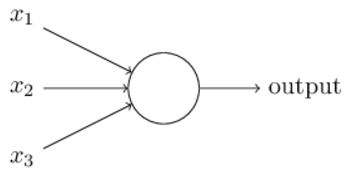
\includegraphics[scale=0.6]{Bilder/perceptron}
	\caption{Percetron mit den Eingaben $x_1, x_2, x_3$ und der Ausgabe $output$.} 
	\label{fig:perceptron} 
\end{figure}
\noindent
Für die Berechnung der Ausgabe werden sogenannte \textit{Weights} $w_n$ mit $n \in \{1, \cdots, n\}$ eingeführt, welche die Gewichtung der jeweiligen Eingabe festlegen. Der Ausgabewerte $\mathtt{output}$ wird mittels der gewichteten Summe $\sum_j w_j x_k$ und einem definierten Grenzwert $\mathtt{threshold}$ bestimmt.
\begin{equation}
	\mathtt{output} := \left\{
	\begin{array}{ll}
 		0 & \displaystyle \mbox{falls}\quad \sum\limits_j w_j x_j \leq \mathtt{threshold} \\[0.5cm]
 		1 & \displaystyle \mbox{falls}\quad \sum\limits_j w_j x_j > \mathtt{threshold}
	\end{array}\right.
\end{equation}
Werden die \textit{Weights} und der \textit{Threshold} variiert, entstehen unterschiedliche Modelle zur Entscheidungsfindung. Hierbei ist zu beachten, dass eine Minimierung des \textit{Thresholds} den binären Ausgabewert 1 mit einer höheren Wahrscheinlichkeit bedingt. \\

\noindent
Der Aufbau des Netzwerks leitet sich aus den unterschiedlichen Modellen der Entscheidungsfindung ab und wird mit Hilfe der Perceptrons abgebildet (siehe Abb. \ref{fig:perceptron_models}).
\begin{figure}[hbt]
	\centering
	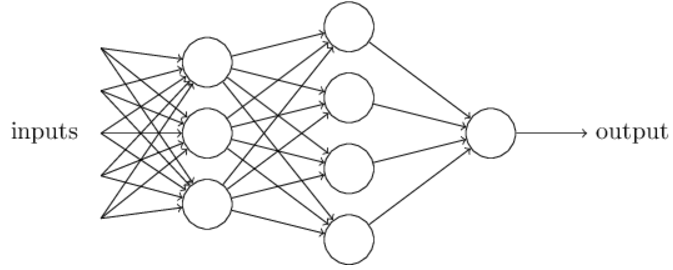
\includegraphics[scale=0.75]{Bilder/perceptron_models}
	\caption{Unterschiedliche Möglichkeiten der Entscheidungsfindung.} 
	\label{fig:perceptron_models} 
\end{figure}
Eine Entscheidungsmöglichkeit wird hierbei durch das Perceptron dargestellt. Weiterhin wird eine Spalte von Perceptrons als \textit{Layer} bezeichnet. Der erste Layer fällt Entscheidungen auf Basis der Eingabewerte, indem er diese abwägt. Jedes Perceptron des zweiten Layers hingegen, wägt für die Entscheidungsfindung die Resultate des ersten Layers ab. Ein Perceptron auf dem zweiten Layer kann somit eine Entscheidung auf einer abstrakteren und komplexeren Ebene durchführen. Auf diese Weise kann sich ein vielschichtiges Netzwerk von Perceptrons in ein anspruchsvolles Modell zur Entscheidungsfindung entwickeln. \\

\noindent
Im folgenden wird die mathematische Beschreibung von Perceptrons vereinfacht, indem Änderungen an der Notation für $\sum_j w_j x_j > \mathtt{threshold}$ vorgenommen werden. Für die Beschreibung der Summe $\sum_j w_j x_j$ werden die Vektoren $w$ und $x$ eingeführt, wodurch sich die Schreibweise $w \cdot x \equiv \sum_j w_j x_j$ ergibt. Des Weiteren wird der $\mathtt{threshold}$ auf die andere Seite der Ungleichung gezogen und erhält die Bezeichnung \textit{Bias}, $b \equiv \mathtt{-threshold}$. 
\begin{equation}
	\mathtt{output} := \left\{
	\begin{array}{ll}
 		0 & \displaystyle \mbox{falls}\quad w \cdot x + b \leq 0 \\[0.2cm]
 		1 & \displaystyle \mbox{falls}\quad w \cdot x + b > 0
	\end{array}\right.
\end{equation}


\section{Sigmoid Neurons}
Für die Entwicklung lernender Algorithmen in einem Netzwerk mit Perceptrons, fällt unsere Betrachtung auf das Beispiel der Erkennung von handgeschriebenen Zahlen. Die Eingabe für das Netzwerk könnten die Raw Pixeldaten der eingescannten Bilder darstellen, welche die handgeschriebenen Zahlen abbilden. Das Ziel an dieser Stelle ist, dass das Netzwerk anhand der \textit{Weights} und \textit{Biases} lernt eine korrekte Klassifizierung der Zahlen vorzunehmen.